\documentclass[12pt]{article}
\setlength{\textwidth}{167mm}
\setlength{\headsep}{0mm}
\setlength{\headheight}{0mm}
\setlength{\textheight}{230mm}
\setlength{\oddsidemargin}{1.6mm}
\setlength{\evensidemargin}{1.6mm}
\setlength{\topmargin}{4.6mm}

\usepackage{chngcntr}
\usepackage{xspace}
\usepackage{graphicx}
\graphicspath{{Images/}}
\usepackage[symbol]{footmisc}


% Astronomical abbreviations (thanks to Dan Huber)
\newcommand{\numax}{\mbox{$\nu_{\rm max}$}\xspace}
\newcommand{\dnu}{\mbox{$\Delta \nu$}\xspace}
\newcommand{\muHz}{\mbox{$\mu$Hz}\xspace}
\newcommand{\teff}{\mbox{$T_{\rm eff}$}\xspace}
\newcommand{\logg}{\mbox{$\log(g)$}\xspace}
\newcommand{\feh}{\mbox{$\rm{[Fe/H]}$}\xspace}
\newcommand{\msun}{\mbox{$\mathrm{M}_{\odot}$}\xspace}
\newcommand{\lsun}{\mbox{$\mathrm{L}_{\odot}$}\xspace}
\newcommand{\mearth}{\mbox{$\mathrm{M}_{\oplus}$}\xspace}
\newcommand{\rsun}{\mbox{$\mathrm{R}_{\odot}$}\xspace}
\newcommand{\kepler}{\emph{Kepler}\xspace}
\newcommand{\tess}{\emph{TESS}\xspace}
\newcommand{\ktwo}{K2\xspace}
\newcommand{\gaia}{\emph{Gaia}\xspace}

\begin{document}
\noindent\textbf{\LARGE{New asteroseismic rotation rates of \emph{Kepler} dwarfs show strong agreement with weakened magnetic braking on the late-age main sequence}}\\

\noindent Oliver J. Hall$^{1,2,3,}$\footnote[1]{Email: \texttt{oliver.hall@esa.int} | Twitter: \texttt{@asteronomer} | GitHub: \texttt{@ojhall94}}
	Guy R. Davies$^{2,3}$, 
	Jennifer van Saders$^{4,5,6}$,
	Martin B. Nielsen$^{2,3}$
	Mikkel N. Lund$^{3}$, 
	William J. Chaplin$^{2,3}$, 
	Rafael A. Garc\'ia$^{7, 8}$, 
	Louis Amard$^{9}$,
	Angela A. Breimann$^{9}$, 
	Saniya Khan$^{2,3}$, 
	Victor See$^{9}$, 
	Jamie Tayar$^{4, 10}$
	\\
	
	% List of institutions
	\noindent $^{1}$ Scientific Support Office, Directorate of Science, European Space Research and Technology Centre (ESA/ESTEC), Keplerlaan 1, 2201 AZ Noordwijk, NL

	\noindent 	$^{2}$ School of Physics and Astronomy, University of Birmingham, Edgbaston, Birmingham, B15 2TT, UK

	\noindent 	$^{3}$ Stellar Astrophysics Centre, Department of Physics and Astronomy, Aarhus University, Ny Munkegade 120, 8000 Aarhus C, Denmark

	\noindent 	$^{4}$ Institute for Astronomy, University of Hawai'i, Honolulu, HI 96822

	\noindent 	$^{5}$ Observatories of the Carnegie Institution for Science, Pasadena, CA 91101

	\noindent 	$^{6}$ Department of Astrophysical Sciences, Princeton University, Princeton, NJ 08544

	\noindent 	$^{7}$ IRFU, CEA, Universit\'e Paris-Saclay, F-91191 Gif-sur-Yvette, France

	\noindent 	$^{8}$ AIM, CEA, CNRS, Universit\'e Paris-Saclay, Universit\'e Paris Diderot, Sorbonne Paris Cit\'e, F-91191 Gif-sur-Yvette, France

	\noindent 	$^{9}$ University of Exeter Department of Physics and Astronomy, Stocker Road, Devon, Exeter, EX4 4QL, UK
	
	\noindent $^{10}$ Hubble Fellow


\vspace{10mm}

\textbf{Studies using asteroseismic ages and rotation rates from star spot rotation have shown that standard age-rotation relations break down roughly half-way through the main sequence lifetime, a phenomenon referred to as weakened magnetic braking. While rotation rates from spots can be difficult to determine for older, less active stars, rotational splitting of asteroseismic oscillation frequencies can provide rotation rates for both active and quiescent stars.\\
We obtained asteroseismic rotation rates of 91 main sequence stars showing high signal-to-noise modes of oscillation.
Using these new rotation rates, along with effective temperatures, metallicities and seismic masses and ages, we built a hierarchical Bayesian mixture model to determine whether the ensemble more closely agreed with a standard rotational evolution scenario \cite{vansaders+pinsonneault2013}, or one where weakened magnetic braking takes place \cite{vansaders+2016}. The weakened magnetic braking scenario was found to be $98.4\%$ more likely for our stellar ensemble, adding to the growing body of evidence for this stage of stellar rotational evolution. This work represents the largest catalogue of seismic rotation on the main sequence to date, opening up possibilities for more detailed ensemble analysis of rotational evolution with \textit{Kepler}.}

%%%%%%%%%%%%%%%%%%%% REFERENCES %%%%%%%%%%%%%%%%%%
\section{Introduction} %500 words
Gyrochronology is the study of the relationship between a star's rotation period and its age. As a star grows older along the main sequence, magnetic winds will cause it to lose angular momentum, slowing it down. Because the loss rate is related to temperature, the rotation period of a young star will rapidly settle on to a plane in age-colour-rotation space \cite{barnes2007}. As a result, knowing the rotation and colour of a star provides an avenue to measure it's age, which can otherwise be difficult to come by, enabling more in-depth studies of stellar populations \cite{leiner+2019,claytor+2019}.

Gyrochronology was previously calibrated on stellar clusters, which have well constrained ages, but only up to roughly $2.5\, \rm{Gyr}$ so far \cite{meibom+2015}. With the launch of the \textit{Kepler} mission \cite{borucki+2010}, ages of main sequence field stars (i.e. not in clusters) became more widely available through asteroseismology, the study of stellar variability \cite{silvaaguirre+2015}. When looking at these stars disagreements were found with gyrochronology beyond the middle of their main sequence lifetime, which could not be reconciled with existing theories \cite{angus+2015, nielsen+2015, davies+2015}. It was proposed that at some stage in a star's evolution it undergoes \textit{weakened magnetic braking} (WMB, \cite{vansaders+2016}), where the efficiency of angular momentum loss rapidly drops, causing stars to keep fast rotation rates that we were not expected in existing gyrochronology relations.

The mechanism by which weakened magnetic braking occurs is  still subject to debate, and may be connected to changes in the magnetic field morphology \cite{reville+2015,garraffo+2016, metcalfe+2019, see+2019}. It may also be explained from an observational point of view. A large scale survey of stellar rotation rates measured using star spots pointed out a lack of slowly rotating stars older then Sun \cite{mcquillan+2014}. As activity reduces with age, older stars with fewer star spots are less likely to have their rotation measured \cite{matt+2015}. The point at which the detection probability drops appears to lie at a similar level of activity to that at which the proposed weakened magnetic braking takes place, pitting these two possibilities against one another \cite{vansaders+2019}.

Determining whether weakened magnetic braking is a true phenomenon or a bias in star spot observations requires new data, which can be provided by asteroseismology. A star's rotation causes modes of oscillation to split into multiplets, making it possible to measure the rate of rotation by measuring oscillation frequencies \cite{ledoux1951}. Asteroseismic rotation is more difficult to obtain than rotation from star spots, but does not require  spots to be visible, meaning that we can measure rotation for quiescent stars that would not have been present in existing catalogues of star-spot rotation. Previous studies have shown that asteroseismic rotation rates probe the near-surface of the star, making them comparable to spot rotation rates, and the perfect avenue to explore whether weakened magnetic braking truly takes place \cite{lund+2014, benomar+2015}. Here, we measured asteroseismic rotation rates of 91 main sequence stars across a broad range of colours and ages, and evaluate this new ensemble to determine whether it agrees more closely with a classical rotational evolution scenario, or one where weakened magnetic braking takes place.\\

\section{Data}

In order to obtain robust asteroseismic rotation rates, we required detections of multiples of both dipole (denoted as $\ell = 1$) and quadrupole ($\ell = 2$) oscillations for each star, of which the latter have significantly lower signal-to noise. Radial oscillations ($\ell = 0$), which are also visible, do not split. In this work, we studied a sample of 95 of the highest signal-to-noise targets observed by \textit{Kepler}, combining the `Kages' \cite{silvaaguirre+2015,davies+2016} and LEGACY \cite{lund+2017, silvaaguirre+2017} catalogues\footnote{For these catalogues the mode extraction through frequency fitting \cite{davies+2016, lund+2017} and modelling using mode frequencies to obtain stellar parameters \cite{silvaaguirre+2015, silvaaguirre+2017} are covered in separate papers.}. A table of parameters taken from these studies, as well as details on how these were obtained, can be found in \textbf{\textit{Methods}}. 

We separated our sample into three categories \cite{garcia+2014}: 64 main sequence stars (MS, $\rm{log(g)} > 4.0\, \rm dex$, $T_{\rm eff} < 6250\, \rm K$); 4 potential sub-giant stars (SG, $\rm{log(g)} < 4.0\, \rm dex$, $T_{\rm eff} < 6250\, \rm K$, which may have begun to evolve off the main sequence, complicating their rotational history\footnote{It should be noted that none of these stars have identified mixed dipole modes, which indicate an evolved structure (see \cite{bedding+2010}).}; and 24 `hot' stars (H, $T_{\rm eff} > 6250\, \rm K$), which lie above the Kraft break, the point at which convective envelopes are tenuous, and angular momentum loss becomes inefficient \cite{kraft1967}. The sample, which can be seen in Figure \ref{fig:sample}, spans surface gravities of $3.8\, \rm{dex} < \rm{log(g)} < 4.6\, \rm{dex}$, temperatures of $5000\, \textrm{K} < T_{\rm eff} <  6700\, \rm{K}$, and ages from $1$ to $\sim 13\, \rm{Gyr}$.

\begin{figure}
	\centering
	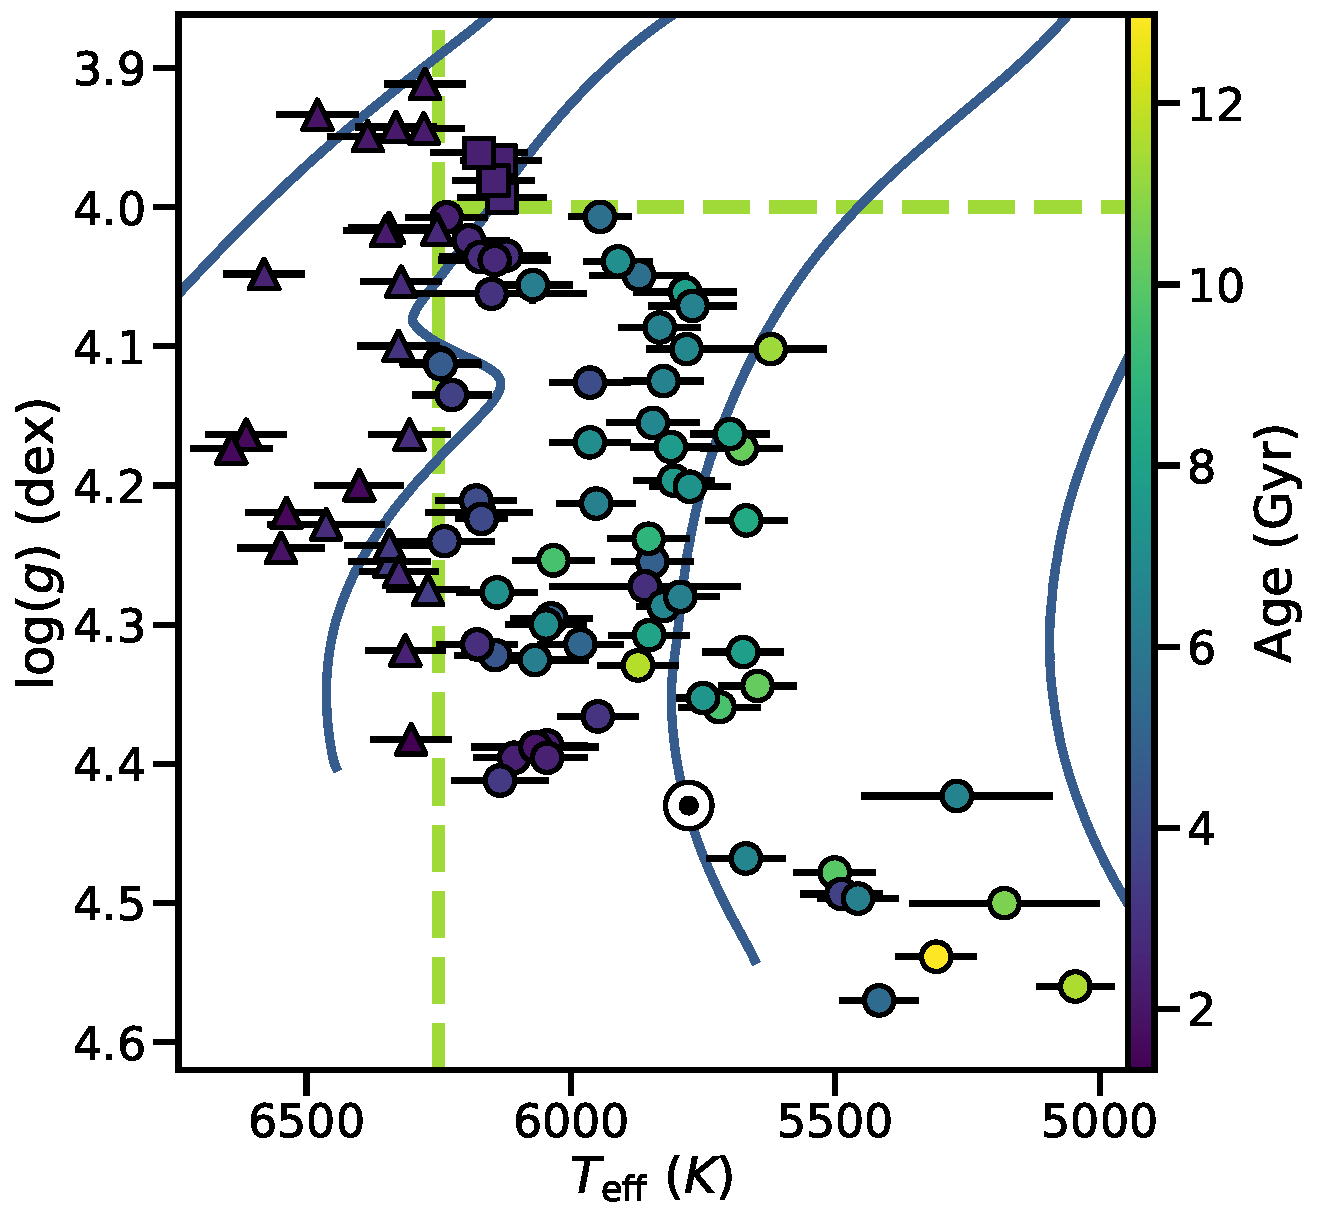
\includegraphics[width=0.8\textwidth]{data.pdf}
	\caption{Our sample of 95 stars from the Kages and LEGACY catalogues coloured by asteroseismic age  \cite{silvaaguirre+2015, silvaaguirre+2017}. The dashed lines indicate our classification boundaries: main sequence (circles, $\teff < 6250\, K$, $\logg < 4\, \rm{dex}$), potential sub-giants (squares, $\teff < 6250\, K$, $\logg > 4\, \rm{dex}$), and `hot' stars (triangles, $\teff > 6250\, K$). The Sun is shown with the `$\odot$' symbol, and has an age of $4.6\, \rm{Gyr}$ \cite{bonanno+frohlich2015
		}. The solid lines are evolutionary tracks generated using MESA \cite{paxton+2017}, for a metallicity of $Z = 0.01493$ and helium content of $Y = 0.26588$. Left to right, they represent masses of $1.5$, $1.25$, $1$ and $0.75\, M_\odot$. Vertical errorbars are too small to be visible.}
	\label{fig:sample}
\end{figure}


\section{Results}
 The `Kages' and LEGACY catalogues that form our stellar sample both performed detailed asteroseismic frequency fitting, but did not report asteroseismic rotation. Here, we repeated the mode frequency fitting with an improved Bayesian model that accounted for rotation in more detail (see \textbf{\textit{Methods}}). We fit our model to \kepler power-spectra of 95 stars, which was successful in 94 cases. We compared our results with both published and unpublished asteroseismic rotation rates, and found that the three stars with the lowest angles of inclination ($< 10^\circ$) were inconsistent with previous work. To some degree this was expected, as  for stars viewed near pole-on the power of the split modes of oscillation are extremely small. We flagged our rotation rates for these stars, and did not use them in the next steps in our analysis, leaving a sample of 91 stars for which we judge our asteroseismic rotation measurements to be robust (for a full justification, see \textit{\textbf{Methods}}).

\section{Discussion}

% The best way to enter references is to use BibTeX:
\bibliographystyle{naturemag}
\bibliography{library.bib} %

\section*{Acknowledgements}

\section*{Methods}

\section*{Author Contributions}


\end{document}